\newpage
\begin{center}
  \textbf{\large 2. АНАЛИЗ НАБОРОВ ПОСЛЕДОВАТЕЛЬНОСТЕЙ}
\end{center}
\refstepcounter{chapter}
\addcontentsline{toc}{chapter}{2. АНАЛИЗ НАБОРОВ ПОСЛЕДОВАТЕЛЬНОСТЕЙ}

\section{Расширение алгоритма PCA-Seq для анализа наборов последовательностей}

До этого момента мы рассматривали алгоритм PCA-Seq исключительно для анализа отдельных последовательностей. Однако гораздо чаще в практике встречаются случаи, когда нам необходимо анализировать несколько последовательностей, сравнивать их между собой, использовать, как исходные данные для задач классификации и регрессии. При этом часто последовательности имеют разную длину, что усложняет применение к ним классических методов предобработки данных или делает их менее эффективными.

Идея нашего метода заключается в повторном применении шагов алгоритма PCA-Seq, тем самым делая возможным анализ нескольких последовательностей. Рассмотрим подробнее, что подразумевается под повторным применением шагов.

Напомним, что при анализе отдельных последовательностей в качестве результата алгоритма мы получаем фазовую траекторию исходной последовательности в пространстве главных компонент. Пример можно увидеть на рисунке~\ref{trajectory} из предыдущей главы.

Пусть мы рассматриваем $Q$ последовательностей $S_1,\ldots,S_Q$ длины \\$K_1,\ldots,K_Q$ соответственно, и по каждой из них проходим скользящим окном с общими фиксированными параметрами $W$ и $T$. Для каждой последовательности получаем $N_i~= \left\lceil\frac{K_i-W}{T}\right\rceil + 1$ фрагментов ($F_{i1},\ldots, F_{iN_i}$). Всего $N = N_1 + \ldots + N_Q$ фрагментов.

Применив PCoA к множеству фрагментов, полученных из всех последовательностей и соединив в нужном порядке точки, относящиеся к одним и тем же последовательностям, мы получим несколько фазовых траекторий, расположенных в общем евклидовом пространстве главных компонент.

Пусть точка $X_{ij}$ соответствует фрагменту $F_{ij}$ ($i \in \{1,\ldots, Q\}$, \\$j \in \{1, \ldots, N_i\}$). Тогда получаем фазовые траектории:

\begin{itemize}
  \item $\hat{T}_1 = X_{11},\ldots,X_{1 N_1}$,
  \item $\hat{T}_2 = X_{21},\ldots,X_{2 N_2}$,
  \item $\ldots$
  \item $\hat{T}_Q = X_{Q1},\ldots,X_{Q N_Q}$.
\end{itemize}

Уже на этом этапе мы получаем наглядное геометрическое представление набора молекулярных последовательностей. Каждая последовательность представляется ломаной, при этом близкие друг другу фрагменты (согласно выбранной метрике) отображаются в близкие друг другу точки, а длины получившихся ломаных пропорциональны длинам исходных последовательностей.

Однако мы можем получить представление последовательностей и в виде точек. Введем метрику $d_T(\hat{F}_i, \hat{F}_j)$, которая будет считать расстояние между фазовыми траекториями (ломаными) разной длины. Тогда мы можем построить матрицу расстояний между фазовыми траекториями и применить к ней PCoA. Тем самым мы получим геометрическое представление для каждой из исходных последовательностей в виде точки в пространстве главных компонент.

Оценим вычислительную сложность такого алгоритма. Положим $K = K_1 +\ldots + K_Q$. Для вычисления фазовых траекторий, как было показано в первой главе (формула \ref{asimp1}), необходимо $O\left(\left(\frac{K}{T}\right)^3\right)$ времени. Далее нам необходимо посчитать матрицу расстояний между траекториями размерности $Q\times Q$. Как будет показано далее, в большинстве используемых нами метрик, необходимо $O(N_i N_j)$ времени, чтобы посчитать расстояние между траекториями длины $N_i$ и $N_j$ соответственно. Положим, что $\overline{N}$~--- средняя длина траектории. Тогда эта часть алгоритма займет $O(Q^2\overline{N}^2)$ времени. Если сделать оценку $Q\overline{N} \approx N \approx \frac{K}{T}$, то можно переписать эту часть, как $O\left(\left(\frac{K}{T}\right)^2\right)$. И наконец, в конце, нам необходимо применить SVD к матрице $Q\times Q$, что займет $O(Q^3)$ времени. Итоговая вычислительная сложность составит $O\left(\left(\frac{K}{T}\right)^3 + Q^3\right)$. Если положить, что $\overline{K}$~--- средняя длина последовательности и $K \approx Q\overline{K}$, то можно записать асимптотику, как

\begin{equation}
  O\left(\left(\frac{Q\overline{K}}{T}\right)^3\right).
  \label{asimp2}
\end{equation}

\section{Выбор метрик для расчета расстояний между фазовыми траекториями}

Пусть даны две траектории: $\hat{T}_i = X_{i1},\ldots,X_{i N_i}$ и $\hat{T}_j = X_{j1},\ldots,X_{j N_j}$. Все точки траекторий расположены в одном евклидовом пространстве размерности $M$. Обозначим для удобства расстояние Пифагора между двумя точками как $d(x, y).$

Первая метрика, которую мы взяли в рассмотрение --- это расстояние Пифагора между двумя средними точками двух траекторий. Пусть\\ $\overline{T_i} = \frac{1}{N_i}\sum_{k=1}^{N_i} X_{ik}$, $\overline{T_j} = \frac{1}{N_j}\sum_{k=1}^{N_j} X_{jk}$. Тогда

$$\text{mean}(i, j) = d(\overline{T_i}, \overline{T_j}).$$

При подсчете этой метрики теряется много информации о траектории: не учитывается набор точек, их порядок и количество. Зато ее вычисление происходит быстро: за $O(N_i + N_j)$ времени.

Следующая метрика --- расстояние Хаусдорфа между двумя множествами:

$$\text{hausdorff}(i, j) = \max\left\{\max_{x\in\hat{T}_i} \min_{y\in\hat{T}_j} d(x, y), \max_{y\in\hat{T}_j} \min_{x\in\hat{T}_i} d(x, y)\right\}.$$

Оно определяет наибольшее из всех расстояний от точки одного множества до ближайшей к ней точки другого множества. Эта метрика уже учитывает все точки траекторий, но не учитывает их порядок, так как метрика введена для множеств. Для ее вычисления необходимо $O(N_iN_j)$ времени.

Также мы ввели собственную вариацию расстояния Жаккара для траекторий:

$$\text{jaccard\_tr}(i, j) = \sqrt{1 - \frac{\|\hat{T}_i \cap \hat{T}_j\|}{N_i + N_j}}.$$

Пусть $X_{ik_1}$~--- точка из траектории $\hat{T}_i$, $X_{jk_2}$~--- точка из траектории $\hat{T}_j$ Так как крайне маловероятно, что точки траекторий будут совпадать, мы считаем, что две точки $X_{ik_1}$ и $X_{jk_2}$ лежат в пересечении $\hat{T}_i$ и $\hat{T}_j$, если $X_{jk_2}$ является ближайшей точкой для $X_{ik_1}$ среди всех точек траекторий $\hat{T}_i$ и $\hat{T}_j$. Эта метрика так же не учитывает порядок точек в траектории. Она считается за $O((N_i + N_j)^2)$

Наконец, рассмотрим расстояние Фреше (frechet), которое в общем виде введено для произвольных кривых и принимает во внимание число и порядок точек. Интуитивно это расстояние часто объясняют через пример человека, выгуливающего собаку. Пусть заданы две траектории: для человека и для собаки. Каждый из них может изменять скорость движения, но не может двигаться назад. Расстояние Фреше между этими двумя траекториями --- это длина кратчайшего поводка, достаточная для того, чтобы и человек, и собака смогли пройти по своим траекториям от начала до конца.

Томас Айтер и Хайкки Маннила ввели \cite{Eiter1994ComputingDF} дискретное расстояние Фреше, которое является аппроксимацией расстояния Фреше для ломаных и рассматривает положение <<поводка>> только в их вершинах. Оно вычисляется при помощи алгоритма динамического программирования за $O(N_iN_j)$.

\section{Задача предсказания термофильности организмов}

Для проверки применимости нашего метода на реальных биологических задачах мы попробовали решить при помощи него задачу предсказания термофильности организма по аминокислотной последовательности его белка.

Изначально коллегами из Лаборатории генетических технологий ИХБФМ СО РАН перед нами была поставлена задача предсказания термостабильности ДНК-полимераз, которые играют ключевую роль в сохранении стабильности генома. ДНК-полимеразы используются и в различных приложениях молекулярной биологии, в частности, в методе полимеразной цепной реакции (ПЦР). Для проведения ПЦР необходимы как раз термостабильные полимеразы \cite{bulygin}. Термостабильным считается фермент у которого период полураспада при температуре 95 °C составляет не менее 10 минут.

К сожалению, обучающая выборка, предоставленная коллегами оказалась очень мала. В ней содержались 9 термостабильных и 5 нетермостабильных достоверно проверенных ДНК-полимераз. Такого количества данных было недостаточно для обучения модели классификации. К тому же большинство полимераз из первого класса относились к одному виду, поэтому их внутривидовое сходство сильно бы <<отвлекало>> обучаемую модель от реальных признаков термостабильности.

По этой причине мы были вынуждены искать другие данные для обучения. Нами была обнаружена модель глубокого обучения DeepTP, разработанная в 2023 году \cite{Zhao2023}, которая предсказывает термофильность или мезофильность организма по аминокислотной последовательности его белка. В открытый доступ выложены обучающие и тестовые выборки модели. Авторы статьи считают термофильным организм, минимальная температура роста которого выше 60 °C. А мезофильным~--- организм, максимальная температура роста которого ниже 37 °C. Модель решает задачу бинарной классификации.

Задача предсказания термофильности организма близка к задаче предсказания термостабильности белка, однако из первого критерия не всегда следует второй. Известны организмы, живущие при повышенных температурах, полимеразы которых работают при таких температурах, но их стабильность значительно снижается при более высоких температурах, поэтому они не могут использоваться в ПЦР \cite{bulygin}.

Тем не менее, обучение такой модели позволит нам проверить наш метод, а также позволит сравнить точность полученной модели с уже имеющимися.

\section{Результаты применения метода}

Обучающая выборка DeepTP состоит из 19 тыс. аминокислотных последовательностей. Кубическая вычислительная сложность нашего алгоритма (формула \ref{asimp2}) не позволила нам применить его к такой большой выборке. Поэтому мы сосредоточились на валидационной выборке этой модели, которая взята из модели TMPred \cite{Meng2022} 2022-го года и состоит из 101 мезофильного и 105 термофильных белков.

TMPpred~--- модель бинарной классификации, основанная на SVM, которая фокусируется на определении признаков, влияющих на термофильность и анализирует набор признаков с помощью улучшенного метода ANOVA, выявляя семь наиболее важных признаков. Ее точность на предоставленной выборке составляет 0.875.

На рисунке \ref{lens} представлена гистограмма распределения длин последовательностей в выборке. Видно, что большинство последовательностей имеют длину 150-200 аминокислот.

\begin{figure}[htb]
  \centering
  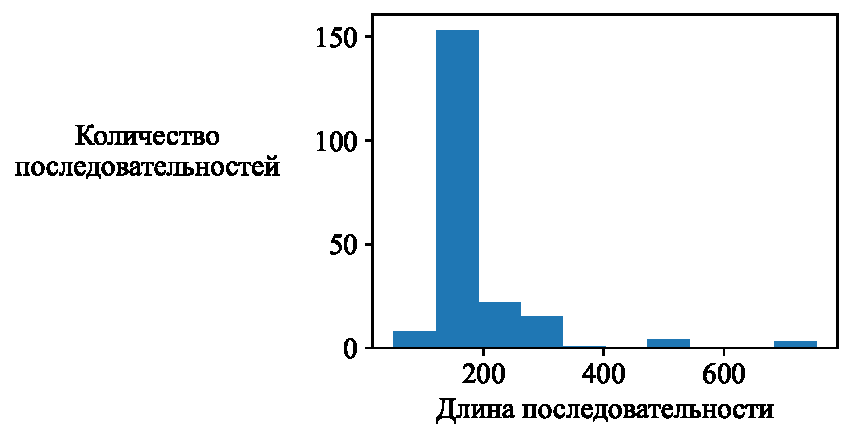
\includegraphics{lens.pdf}
  \caption{Гистограмма распределения длин последовательностей в выборке}
  \label{lens}
\end{figure}

В качестве параметров начального алгоритма для вычисления фазовых траекторий мы взяли следующие значения:

\begin{itemize}
  \item размер скользящего окна $W = 20$,
  \item шаг скользящего окна $T = 5$,
  \item метрика --- расстояние Пифагора между частотными характеристиками (pythagoras), 
  \item размер $L$-граммы $L = 1$ (т. е. считались частотные характеристики аминокислот, Amino Acid Composition).
\end{itemize}

На рисунке \ref{dispersions-tr} представлены распределения дисперсий главных компонент, полученные разными метриками. Как мы видим, по этому критерию расстояние между средними точками траекторий является самым эффективным. Однако, как мы помним, при использовании этой метрики теряется большое количество информации о траекториях, поэтому логично, что для нее получилось объяснить большую долю дисперсии при помощи меньшего количества компонент.

\begin{figure}[htb]
  \centering
  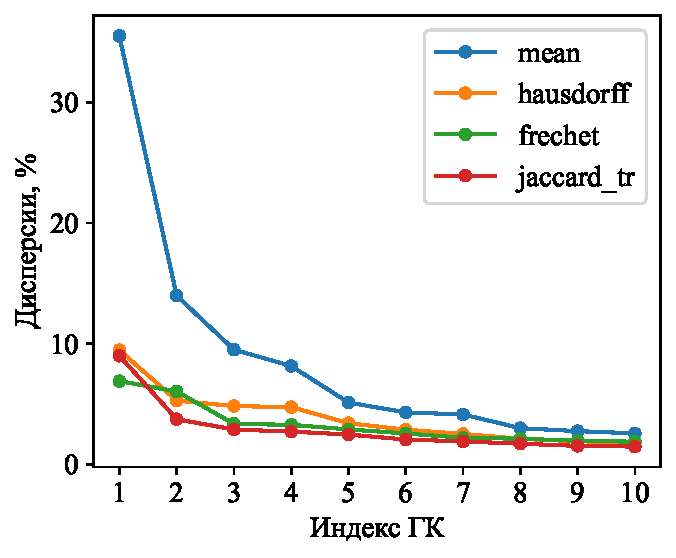
\includegraphics{dispersions-tr.pdf}
  \caption{Распределения дисперсий первых десяти главных компонент для различных метрик между фазовыми траекториями}
  \label{dispersions-tr}
\end{figure}

Сравним эффективность метрик, использовав получившиеся векторные представления фазовых траекторий как входные данные (векторы признаков) для моделей бинарной классификации.

Мы применили несколько популярных методов машинного обучения, таких как
\begin{itemize}
  \item K ближайших соседей (KNN),
  \item метод опорных векторов (SVM),
  \item дерево решений (Decision Tree),
  \item случайный лес (Random Forest),
  \item градиентный бустинг (Gradiend Boosting).
\end{itemize}

Мы оценивали точность моделей при помощи перекрестной проверки (cross validation), несколько раз применяя метод K-Fold (Repeated K-Fold).

В таблице \ref{table-accuracy} представлены результаты обучения моделей на наборах данных, полученных при помощи разных метрик.

\begin{table}[htb]
  \centering{
    \begin{tabular}{|m{60mm}|m{22mm}|m{22mm}|m{22mm}|m{22mm}|}
      \hline
      \backslashbox[60mm]{\textbf{классификатор}}{\textbf{метрика}} & \textbf{mean} & \textbf{hausdorff} & \textbf{jaccard\_tr} & \textbf{frechet}\\
      \hline
      KNN	& 0.858 & 0.947 & 0.861 & 0.816 \\
      SVM & 0.869 & \textbf{0.968} & 0.826 & 0.877 \\
      Decision Tree & 0.79 & 0.913 & 0.821 & 0.764 \\
      Random Forest & 0.848 & 0.96 & 0.87 & 0.844 \\
      Gradient Boosting & 0.843 & 0.958 & 0.845 & 0.833 \\
      \hline
    \end{tabular}
  }
  \caption{Точность моделей бинарной классификации, обученных на данных, полученных разными метриками}
  \label{table-accuracy}
\end{table}

Как можно заметить, метрика Хаусдорфа показала значительно более высокий результат, чем остальные. При использовании метода опорных векторов и нашего алгоритма предобработки данных с метрикой Хаусдорфа точность модели составила 0.968. Точность модели TMPred, которая тоже использует метод опорных векторов, составляет 0.875. Можно сделать вывод, что благодаря нашему алгоритму предобработки, удалось увеличить точность модели на 9.3\%.
